\documentclass[10pt,letterpaper]{article}
\usepackage[utf8]{inputenc}
\usepackage[T1]{fontenc}
\usepackage{amsmath}
\usepackage{amsfonts}
\usepackage{amssymb}
\usepackage{graphicx}
\usepackage{float}
%\usepackage{subfigure}
\usepackage{subcaption}
\usepackage{xcolor}
\definecolor{mblue}{rgb}{0.1, 0.3, 1.0}
\newcommand{\mfont}[1]{{\fontfamily{qcr}\selectfont #1}}
\usepackage[colorlinks=true,linkcolor=blue,urlcolor=black,citecolor=blue]{hyperref}


\begin{document}
	\section*{An  internal flows problem in OpenFOAM}
Consider the geometry given in Figure \ref{fig:geo}. Assume an inlet velocity of $7.5\; m/s$, fluid density of $ 1\;kg/m^3$, and kinematic viscosity of $1.5 \;m^2/s$. Use snappyHexMesh or cfMesh to mesh the provided stl files (depicted above). Set up a simpleFoam simulation to process and report the following results.

\begin{figure}[H]
	\begin{center}
		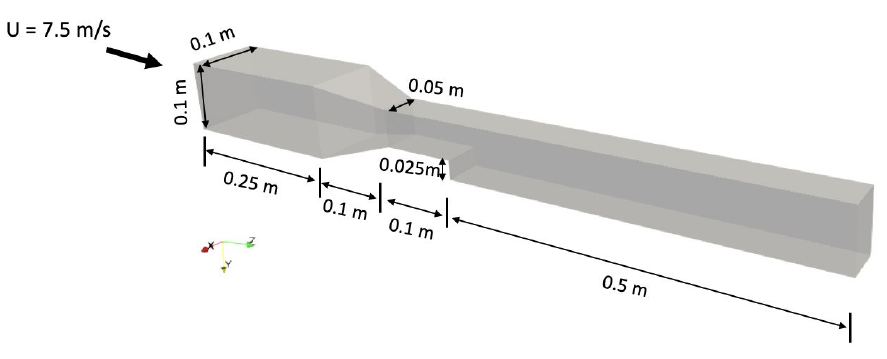
\includegraphics[width=.9\linewidth]{geo.png}
	\end{center}
	\caption{Geometry of the problem}
	\label{fig:geo}
\end{figure}

	{
	\color{mblue}
	Disclaimer: results presented in this report are for the sole purpose of demonstration and are not validated.
}\\

	


\begin{figure}[H]
	\centering	
	\begin{subfigure}{0.7\columnwidth}	
		\centering
		\includegraphics[width=1.0\textwidth]{mesh1.png}
	\end{subfigure}
	\begin{subfigure}{0.7\columnwidth}	
		\centering
		\includegraphics[width=1.0\textwidth]{mesh2.png}
	\end{subfigure}
\caption{Visual details of the generated mesh for the input geometry via  \mfont{snappyHexMesh} }
\end{figure}

\begin{itemize}
	\item Total pressure drop across the domain
	
		{		\color{mblue}
		This is reported by the \mfont{Allrun} script, see also Figure \ref{fig:p}
		}
	\begin{figure}[H]
		\begin{center}
			\includegraphics[width=.7\linewidth]{pressureDrop.png}
		\end{center}
		\caption{Pressure distribution in the domain}
		\label{fig:p}
	\end{figure}
	\item Reattachment point after the backward facing step
	
	{\color{mblue}
		Reattachment point is computed through the wall shear stress and when $\frac{\partial \boldmath u}{\partial z}$ changes sign, see also Figure \ref{fig:reattachment}. 
	}
\begin{figure}[H]
		\begin{subfigure}{0.8\columnwidth}	
		\centering
		\includegraphics[width=1.0\textwidth]{reattchmentLength2.png}
	\end{subfigure}
	\begin{subfigure}{0.8\columnwidth}	
		\centering
		\includegraphics[width=1.0\textwidth]{reattchmentLength1.png}
	\end{subfigure}
	\caption{Estimation of the reattachment length through the wall shear stress (top), and Illustration of the size of the main vortex through velocity streamlines (bottom). }
	\label{fig:reattachment}
\end{figure}

	\item Streamlines emanating from the inlet of the domain
		{\color{mblue}
		 See Figure \ref{fig:streamlines} which can be generated from \mfont{streamLines} post processing utility, see also the \mfont{Allrun} and \mfont{system\slash controlDict\slash streamLines}  scripts.  
	}
	\begin{figure}[H]
		\begin{center}
			\includegraphics[width=.9\linewidth]{streamLines.png}
		\end{center}
		\caption{Streamlines emanating from the inlet of the domain}
		\label{fig:streamlines}
	\end{figure}

\end{itemize}


\section*{Key Questions}
\noindent
\begin{itemize}
	\item How does the meshing procedure and set up change if only the total pressure drop is
	desired?
	{
		\color{mblue}
		If only the total pressure drop is desired, there is not any real post-processing involved and we can just rely on \mfont{system\slash controlDict\slash pressureDifferencePatch} to compute the pressure drop and ignore the command line inputs of \mfont{Allrun} script related to streamLines. The meshing procedure and the rest of the set up do not change
	}
	\item  How would the meshing procedure change for different inlet velocities and fluid
	properties?
		{
		\color{mblue}
	Depending on the flow regime (laminar/turbulent)  that is dictated by the flow velocity and the fluid properties such as density and viscosity through the Re number, the underlying mesh may not need to include very thin boundary cells at the walls (laminar flow) or may need to be extra conservative on the size of the closest cell to the wall (turbulent flows where wall functions are used). In this case, one can compute the necessary spacing through $y^+$ calculators (see \href{https://www.pointwise.com/yplus/}{this link  for instance}) and apply the necessary spacing in the \mfont{addLayersControls} section of \mfont{system\slash snappyHexMeshDict}.
	}

	\item How would you encapsulate this meshing procedure into a software workflow to
	automatically write the requisite meshing files? More specifically, what CAD, fluid, and
	boundary inputs are needed? And what output meshing parameters are they used to
	determine?
	{
		\color{mblue}
		Sorting out all the meshing criteria will be a pre-processing stage to meshing. In such a stage, the bounding volume of the domain is computed (through the CAD files) with an approximate size of cells that matches a user-defined mesh resolution and is subsequently used in \mfont{system\slash blockMeshDict} for creating the background mesh.  Inlet and outlet patch(es) are asked to be imported by the user via ply/stl files and are fed into lists that consequently make it into the \mfont{geometry} section of \mfont{system\slash snappyHexMeshDict}. The inlet/outlet property of each (set of) patch(es) are translated into the boundary conditions defined in \mfont{0.org} files for pressure, velocity and turbulent variables.
	}
	\item What are other features and capabilities we can build leveraging snappyHexMesh,
	cfMesh, and/or OpenFOAM to simplify simulations for design engineers?
		{
		\color{mblue}
		In many cases, design engineers do not exactly know the final setup in advance and look for some general guidelines. In these cases, it will be very valuable to allow users to define a range for a parameter. For instance, an engineer may be looking to select a pump for an application for which the domain geometry is not fully specified. This is a very tedious task even for an experienced CFD engineer. In this scenario, making it easy for them to run a batch of simulations on the cloud in parallel to find an optimum design is very valuable and powerful. OpenFOAM and its many applications and utilities makes it easy to leverage CFD for such as tasks. 
		}
	
\end{itemize}
	
\end{document}